





  In the following diagram, what is $x$?
\begin{center}
 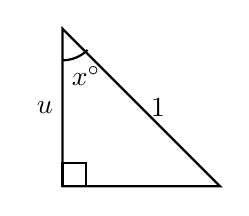
\begin{tikzpicture}
 
 \draw (0,0) --(2,0)--(0,2)--cycle  [thick,-,>=latex];
 \draw (0,0) --(0,.3)--(.3,.3)--(.3,0)--cycle  [thick,-,>=latex];
\draw[thick] (0,1.60) arc (270:315:.45);

  \draw node[below] at (.3,1.65) {$x^\circ$};
  \draw node[left] at (0,1) {$u$};
   \draw node[right] at (1,1) {$1$};
\end{tikzpicture}
\end{center}




\ifsat
	\begin{enumerate}[label=\Alph*)]
		\item    $\arctan\left(\frac{u}{1-u^{2}}\right)$
		\item   $\arctan\left(\frac{1}{1-u^{2}}\right)$ 
		\item  $\arctan\left(\frac{u}{\sqrt{1-u^{2}}}\right)$ 
		\item $\arctan\left(\frac{\sqrt{1-u^{2}}}{u}\right)$ % 
	\end{enumerate}
\else
\fi

\ifacteven
	\begin{enumerate}[label=\textbf{\Alph*.},itemsep=\fill,align=left]
		\setcounter{enumii}{5}
		\item    $\arctan\left(\frac{u}{1-u^{2}}\right)$
		\item   $\arctan\left(\frac{1}{1-u^{2}}\right)$ 
		\item  $\arctan\left(\frac{u}{\sqrt{1-u^{2}}}\right)$ 
		\addtocounter{enumii}{1}
		\item $\arctan\left(\frac{\sqrt{1-u^{2}}}{u}\right)$ % 
		\item $\arctan\left(\frac{\sqrt{u^{2}-1}}{u}\right)$ 
	\end{enumerate}
\else
\fi

\ifactodd
	\begin{enumerate}[label=\textbf{\Alph*.},itemsep=\fill,align=left]
		\item    $\arctan\left(\frac{u}{1-u^{2}}\right)$
		\item   $\arctan\left(\frac{1}{1-u^{2}}\right)$ 
		\item  $\arctan\left(\frac{u}{\sqrt{1-u^{2}}}\right)$ 
		\item $\arctan\left(\frac{\sqrt{1-u^{2}}}{u}\right)$ % 
		\item $\arctan\left(\frac{\sqrt{u^{2}-1}}{u}\right)$ 
	\end{enumerate}
\else
\fi

\ifgridin
 $\arctan\left(\frac{\sqrt{1-u^{2}}}{u}\right)$ % 

\else
\fi

